


\section{Experimentación}
\hfill \break
Para cada filtro y en cada experimento usamos dos muestras de imágenes. Una muestra es generada al azar, o sea el valor de cada píxel de la imagen es determinado de forma azarosa, mientras que en la otra todos sus píxeles tienen el mismo valor, típicamente negro (00000000h) salvo que se indique lo contrario. Usamos dos muestras para mostrar dos casos extremos, uno en que los píxeles están fuertemente relacionados (la imagen constante) y otro en el que no (la imagen aleatoria), y poder ver si hay presente alguna optimización por parte del procesador en alguno de los casos. 
\hfill \break
Como la variación es muy grande entre mediciones, decidimos realizar 100 de estas por cada muestra. Una vez obtenidos los datos nos quedamos con las 10 más chicas y calculamos el promedio. No podemos asegurar que todos los outliers sean removidos de esta forma, pero consideramos que es un método lo suficientemente estable ya que podamos bastantes valores (el 90\%). 
\hfill \break
La métrica que usaremos en todos los casos para comparar la performance de las implementaciones sera ticks por píxel. Consideramos que es una forma justa de comparar dos implementaciones ya que como usan una cantidad de memoria constante (las de Assembler usan solo registros y las de C usan una cantidad fija de variables), lo único que diferencia la performance de ambas es el tiempo de ejecución. Por lo tanto si una implementación requiere menos ticks en la gran mayoría de los casos, es entonces una implementación cuya performance es superior. Si se nos escapa la palabra rápido, o menos tiempo, nos estamos refiriendo a esto, también. 
\hfill \break
\subsection{Cropflip}
\hfill \break
Para este filtro realizamos dos experimentos. El primero consta en medir muestras variando el ancho y alto de estas. De aquí podremos observar como influyen ambos parámetros. El segundo experimento consta en tomar muestras cuadradas e ir incrementando el tamaño. Con este experimento queremos determinar si hay alguna caída de performance al incrementar el volumen de los datos. En ambos casos fijamos los parámetros para que no haya recorte, ya que recortar es equivalente a aplicarle el filtro una imagen de tamaño más chico. (si usamos recorte en alguna descripción nos estaremos refiriendo a imagen de menor tamaño)
La cantidad de accesos de memoria en el c es de cuatro por cada pixel (sino se involucra la cache, una para cada indice de la matriz de destino y entrada). En el caso de que la cache este caliente, el desempeno se vera flanqueado por la velocidad que le toma al procesador realizar los llamados a cache, cuatro veces por pixel, hasta terminal la imagen. En caso de estar fria, se le agregara el tiempo que de ingresos a memoria hasta que la cachese llene. Por supuesto, todo esto se ve limitado por un tamano de imagen que sea capaz de guardar todos sus pixeles en la cache, sino, se tendra que pagar el costo de vaciarla. 
\hfill \break
Hipótesis: Nuestras hipótesis al primer experimento son que al aumentar el ancho y alto de las muestras tomadas, la cantidad de tiempo de las mediciones sera mayor, y, como la implementación de assembler procesa de a 4 píxeles y la de c de a uno x ciclo,  el assembler sera 4 veces mas rápido.
En cuanto al segundo experimento, creemos que incrementar el volumen de los datos a procesar aumente el tiempo de procesamiento, pero debería mantener la diferencia postulada anteriormente. 
Una hipótesis adicional en ambos casos es que, como al shiftear en cropflip no se toma en cuenta el color e la imagen, no tendría que haber mucha diferencia entre las imágenes constantes y las generadas aleatoriamente
\hfill \break
 Los resultados los mostramos en los siguientes gráficos:
 
 \begin{figure} [H]
  \centering
  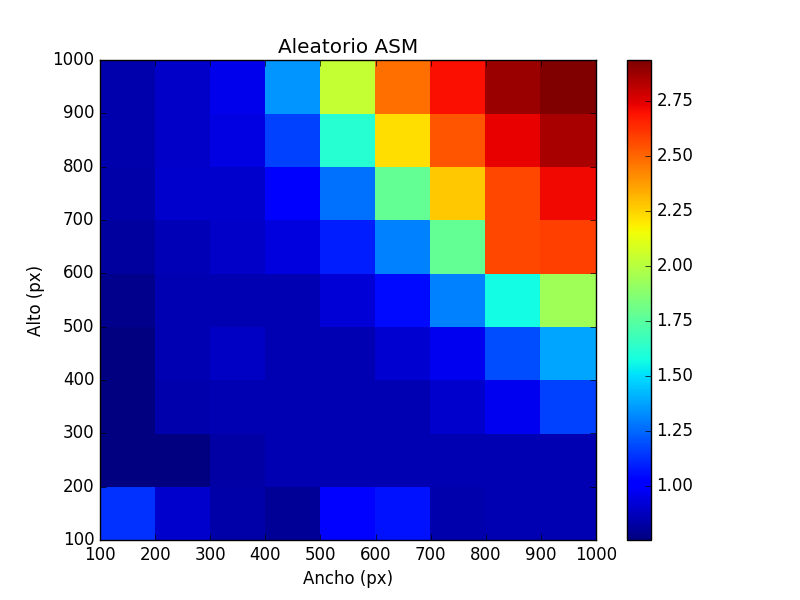
\includegraphics[width=0.8\textwidth]{recursos/aleatoriocropflipasm.png}
    \caption{ Cropflip en imagenes aleatorias de distintos tamaños con assembler }
\end{figure}
 
 \begin{figure} [H]
  \centering
  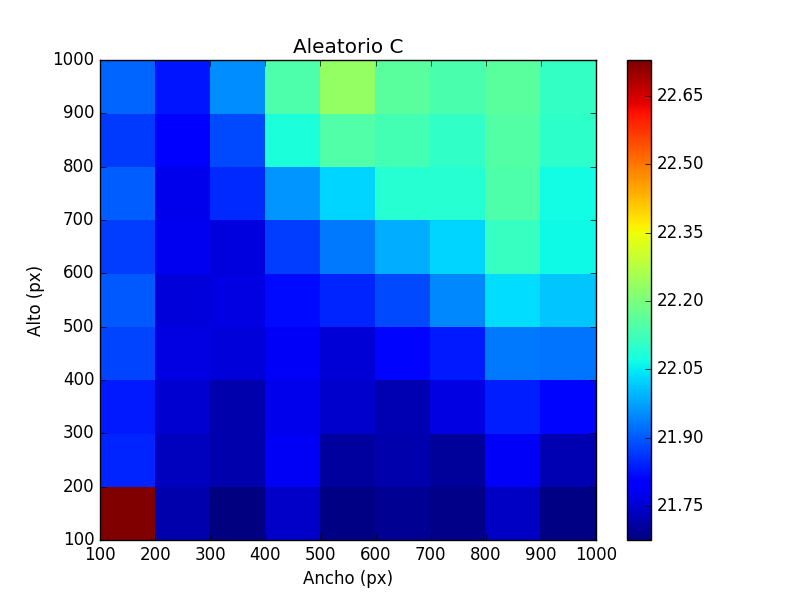
\includegraphics[width=0.8\textwidth]{recursos/aleatoriocropflipc.png}
    \caption{ Cropflip en imagenes aleatorias de distintos tamaños con C }
\end{figure}
 
 
\hfill \break
En el primer experimento, podemos notar la diferencia de performance entre el c y assembler viendo las barras de color, que mientras van de 1 a 2,75 en assembler, van de  22.16 a 21.68 es c, varias veces mas (de hecho, mas de cuatro). En el aleatoria assembler, vemos como va aumentando los ticks por píxel a medida que la imagen se hace mas grande. En el aleatorio c, mientras que al principio (por cache sin datos) tarda mas que nunca, luego su diferencia de performance al aumentar la imagen es menor a la del assembler, (por cache y por que es un proceso mas uniforme de acceso con una estructura definida (matriz) con un tiempo de acceso, en vez de el recorrido por punteros en assembler. De todas maneras, el assembler es mas efectivo
\hfill \break

\begin{figure} [H]
  \centering
  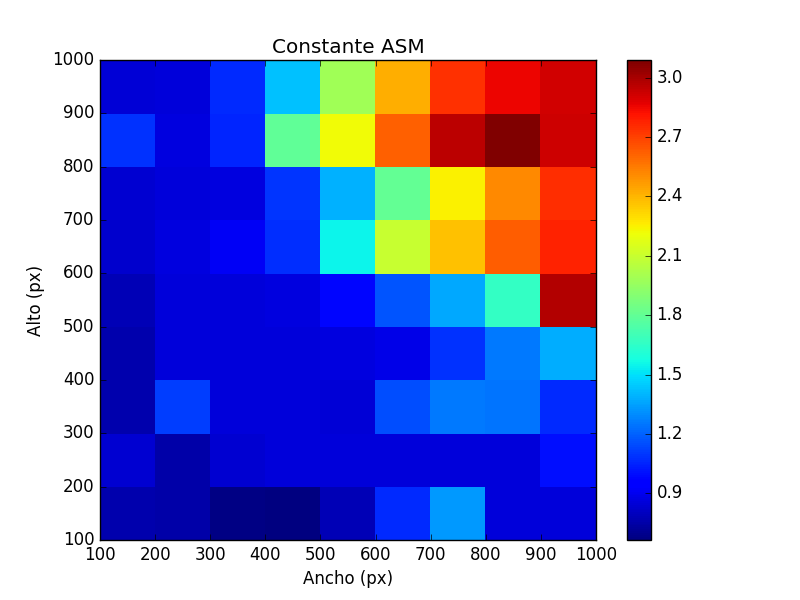
\includegraphics[width=0.8\textwidth]{recursos/constantecropflipasm.png}
    \caption{ Cropflip en imagenes constantes de distintos tamaños con assembler }
\end{figure}
 
 \begin{figure} [H]
  \centering
  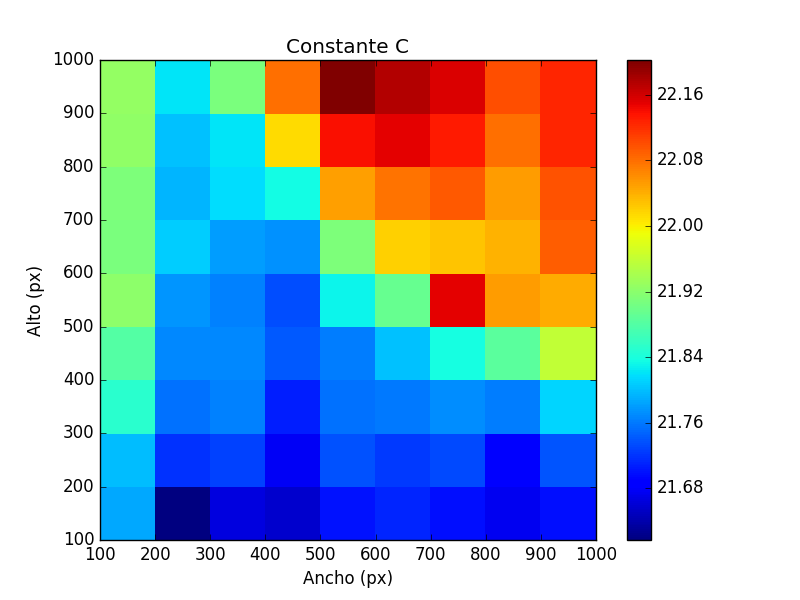
\includegraphics[width=0.8\textwidth]{recursos/constantecropflipc.png}
    \caption{ Cropflip en imagenes constantes de distintos tamaños con C }
\end{figure}
 


Aquí están las constantes de assembler y c con este mismo experimento. Al assembler no hay mucha diferencia, pero en el c la hay, tanto que la optimización de ticks del aleatorio no es aprovechada.
\hfill \break
con respecto al segundo experimento

 \begin{figure} [H]
  \centering
  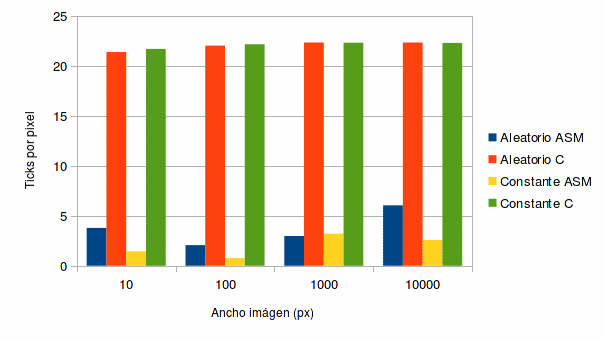
\includegraphics[width=0.8\textwidth]{recursos/cropflipexp2.png}
    \caption{ Comparacion performance assembler vs c, imagenes cuadradas de distintos tamaños  }
\end{figure}
 


\hfill \break
Como podemos ver en el gráfico, están los ticks por píxel de las corridas de assembler y c, dados imágenes cuadradas, donde vamos aumentando su tamaño, y realizamos siempre el mismo recorte. 
Podemos notar que al aumentar el tamaño de imagen, los ticks por píxel de todas las implementaciones c aumentan, así que esa parte de la teoría es correcta. En las implementaciones assembler se da la peculiaridad de que el 100 y 1000 tardan menos que el de 10, en parte se debe a la cache, (una implementacion que es un poco mas grande a 10 aprovecha la cache mas, tal vez 10 es demasiado chico), podemos ver que de 100 en adelante, se cumple para el aleatorio.  
        En cuanto a la relación de tiempos entre el c y el assembler, la menor diferencia que hubo fue entre la implementación de la imagen de 10000x10000, y es un poco menos de 4 veces el tiempo del assembler, pero igualmente una diferencia de 3 veces por lo menos. Como hemos notado antes, no hay bastante diferencia  entre la imagen constante y la no constante en el c, pero nos sorprende la diferencia que se aprecia de este tipo en el assembler en las imágenes.   
         
 \hfill \break
En conclusión, tanto el usar imágenes mas grandes, como el pedir dos recortes, uno mas grande que otro sobre dos imágenes de igual tamaño, hará que los ticks de píxeles aumenten. Un recorte de determinado tamaño tardara mas en una imagen constante que una aleatoria, pero si aumentamos el tamaño de  recorte la diferencia deisminuira. 
\hfill \break
\subsection{Sepia}
Para este filtro vamos a realizar dos experimentos. Son los mismos dos experimentos realizados para cropflip, pero con distintas hipótesis.
\hfill \break
 
   Vamos a decir que el juego de los tamaños de agarrar imágenes cuadradas tenia mas sentido en el cropflip, por lo que solo se hará el análisis con las distintas imágenes constantes y de tamaño. 
   \hfill \break
   Hipótesis:  Nuestras hipótesis son que el tamaño de la imagen hace que tarde mas, y que la imágenes constantes son mas rápidas de procesar que las aleatorias.
   
   
   \begin{figure} [H]
  \centering
  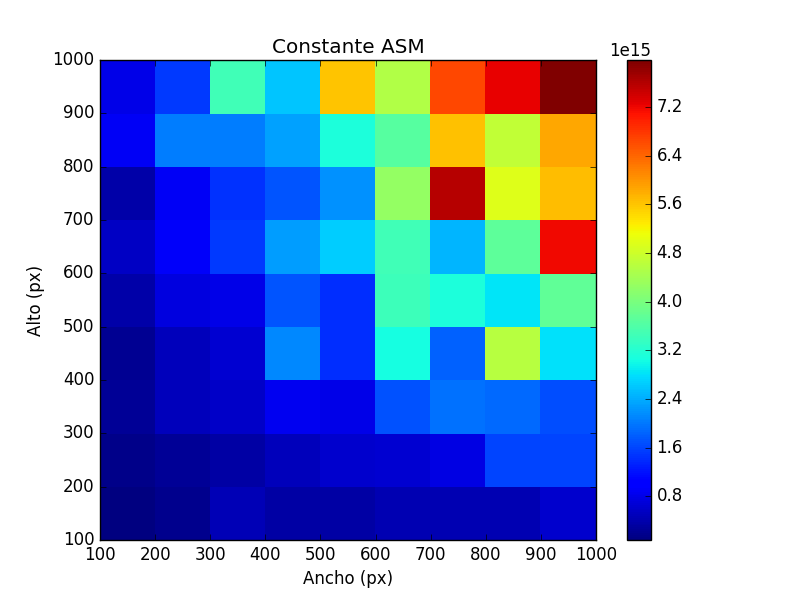
\includegraphics[width=0.8\textwidth]{recursos/constantesepiaasm.png}
    \caption{ Sepia en imagenes constantes de distintos tamaños con assembler }
\end{figure}
 
 \begin{figure} [H]
  \centering
  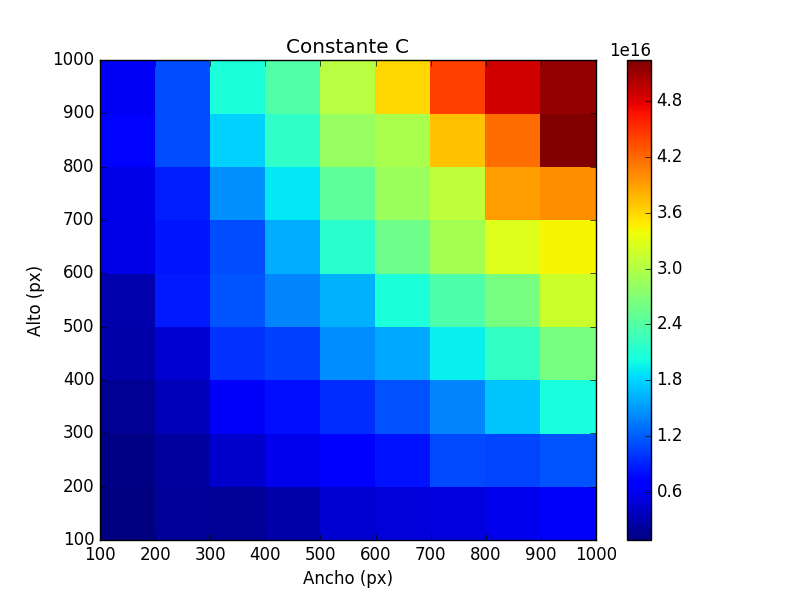
\includegraphics[width=0.8\textwidth]{recursos/constantesepiac.png}
    \caption{ Sepia en imagenes constantes de distintos tamaños con C }
\end{figure}
 
   
   \hfill \break
   
   
   Podemos notar que  el aumento de ticks por píxel en el c de la imagen constante es proporcional a su tamaño uniformemente (con este digo, la variación es constante y proporcionada al incremento), no solo eso, es mas rápido. que el assembler, ( o tal vez no, porque aunque la escala de color de assembler es mayor  hay mas cuadrados con menor escala); pero es alucinadamente rapido. Esto se debe a tener que replicar el mismo resultado sin tener que hacer cuentas, por acceder siempre a iguales datos, ya el procesador pone el resultado; o por estar en el periodo alto de la curva de la cache, si la entrada fuera mas grande, la caché se empezaría a vaciar y el rendimiento caería.
   
   
    \begin{figure} [H]
  \centering
  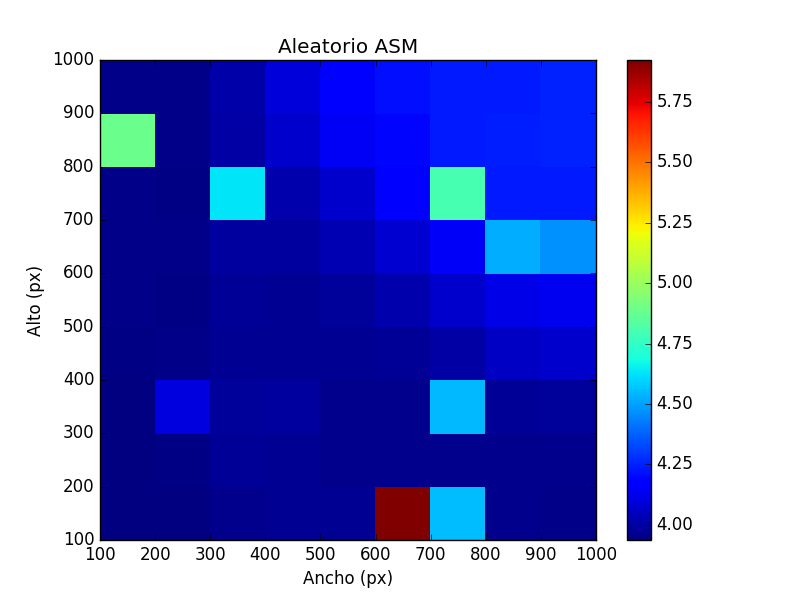
\includegraphics[width=0.8\textwidth]{recursos/aleatoriosepiaasm.png}
    \caption{ Sepia en imagenes aleatorias de distintos tamaños con assembler }
\end{figure}
 
 \begin{figure} [H]
  \centering
  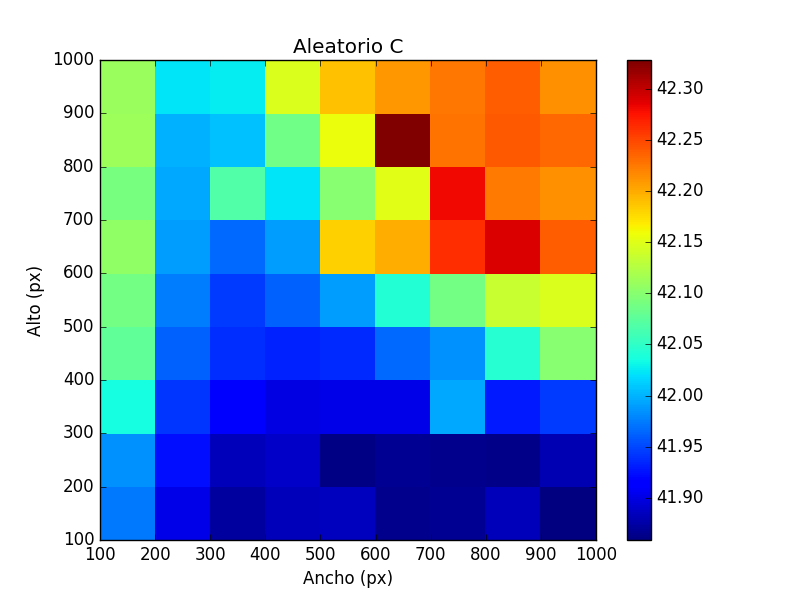
\includegraphics[width=0.8\textwidth]{recursos/aleatoriosepiac.png}
    \caption{ Sepia en imagenes aleatorias de distintos tamaños con C }
\end{figure}

   
   \hfill \break
 Ahora vemos el comportamiento de las implementaciones con las imágenes aleatorias. La diferencia de tiempos en el caso de c comparado a la  uniforme es muy significativa. (al igual que con la del assembler) Notar 
que por el contrario, a la implementación assembler es mas eficiente de esta manera,  por que, como son imágenes de puro negro, las sumas en assembler generalmente tienen que ser saturadas, o lidiar con los carries, o por las multiplicaciones de punto flotante de números mas grandes.
\hfill \break
Conclusiones: El programa c performa mejor si el tamaño de imagen es determinado y constante que el assembler, pero en cualquier otro caso el assembler es mucho mas rápido. Las imágenes aleatorias son mas fáciles para el assembler que las constantes (negra). 
\hfill \break
\subsection{LDR}
\hfill \break
Para este filtro vamos a realizar un experimento. Es el primer  experimento realizado para cropflip, pero con distintas hipótesis.
\hfill \break
Hipótesis: En este filtro cambiamos paleta, al igual que en sepia, pero el cambio de paleta no es independiente de cada píxel, si no que es afectado por los píxeles rondeantes. Tomando esto en cuenta, nos parece lógico pensar que si la imagen es constante, el rendimiento se vera afectado solo por las dimensiones de la imagen, y en el aleatoria el tiempo variara tanto por las dimensiones como por el contenido, pudiendo ser en casos menor a la de la constante. El ldr en asm implementado ahorra muchos usos a memoria por rehusar datos cargados en el ciclo anterior, optimización que el assembler no posee, por lo que el assembler entra la mitad de veces a memoria por fila, lo que, a mayor cantidad de filas, hace que sea menor; en cualquier caso, sera siempre mejor 8 veces (4 por cantidad de píxeles por vez. 4 x memoria). 
Se ven aqui los graficos del experimento:


 \begin{figure} [H]
  \centering
  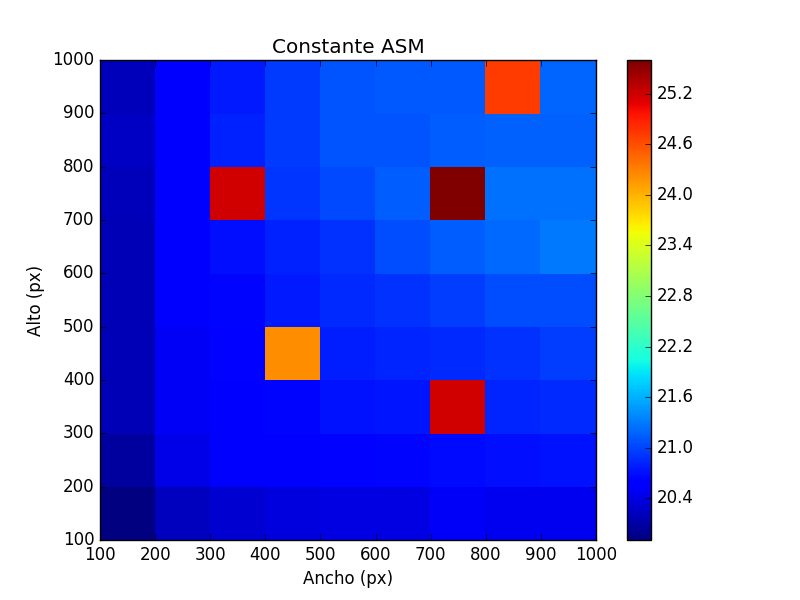
\includegraphics[width=0.8\textwidth]{recursos/constanteldrasm.png}
    \caption{ Ldr en imagenes constantes de distintos tamaños con assembler }
\end{figure}
 
 \begin{figure} [H]
  \centering
  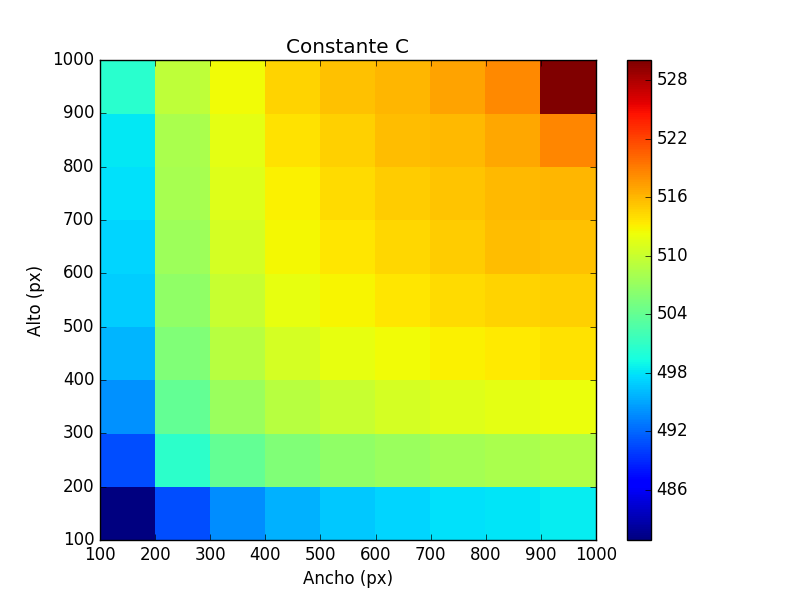
\includegraphics[width=0.8\textwidth]{recursos/constanteldrc.png}
    \caption{ Ldr en imagenes constantes de distintos tamaños con C }
\end{figure}
 
   


   
\hfill \break
Aquí vemos el c y assembler con la figura constante, como podemos nota, el c de nuevo de una distribución bastante uniforme , aunque, comparado con el sepia, en esta ocacion aumentar el tamaño aumenta mas la complejidad, si la otra aumentaba por una constante, esta lo hace de manera cuadrática) eso se debe a que la formula realizada requiere píxeles vecinos. Otra diferencia con el sepia es que esta vez los tiempos no fueron mágicamente menores a los del assembler, por lo mismo de antes. 
El assembler muestra una performance 8 veces mas rápida (de hecho, 16 veces + rápida) y el tiempo del filtro parece casi el mismo sin importar el tamano. Esto se debe a que no elegimos un tamano de imagen lo suficientemente alto, pero que al aumentar como lo hicimos la imagen no se viera afectado en si la rapidez demuestra que se optimiza mucho aprovechando los vecinos de veces anteriores.
\hfill \break

 \begin{figure} [H]
  \centering
  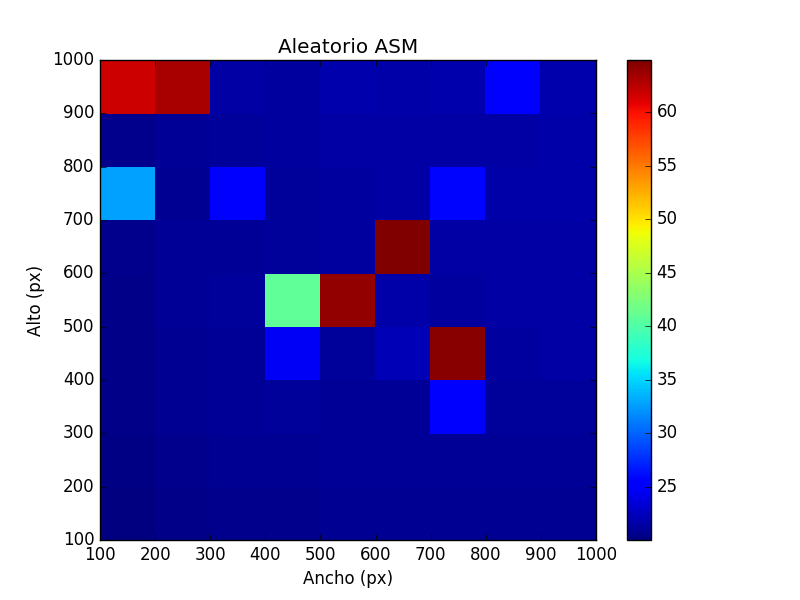
\includegraphics[width=0.8\textwidth]{recursos/aleatorioldrasm.png}
    \caption{ Ldr en imagenes aleatorias de distintos tamaños con assembler }
\end{figure}
 
 \begin{figure} [H]
  \centering
  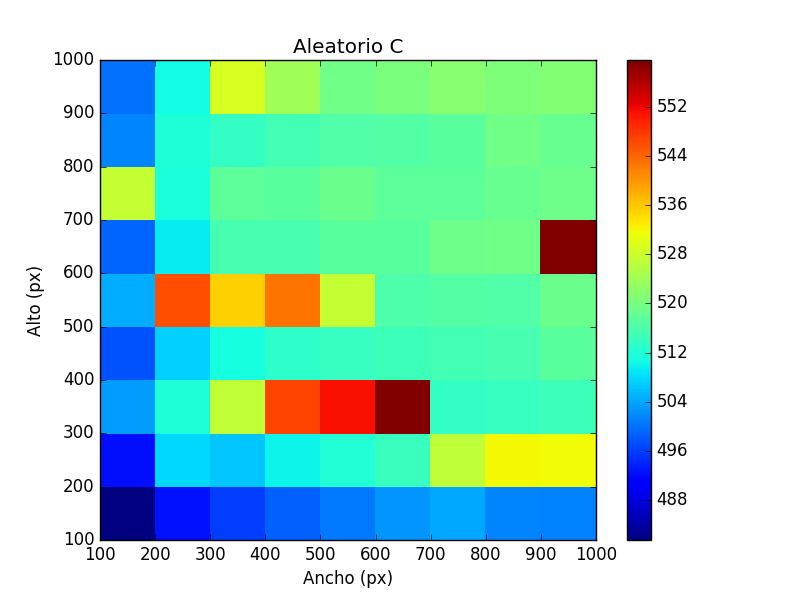
\includegraphics[width=0.8\textwidth]{recursos/aleatorioldrc.png}
    \caption{ Ldr en imagenes aleatorias de distintos tamaños con C }
\end{figure}
 



Aquí vemos el c y el assembler con la figuras aleatorias, aquí el assembler es incluso mas rápido. en la mayoría de los casos, creemos que porque el contenido afecta lo las imágenes, asiéndolas mas fáciles de usar en cuentas y procesar. En cuanto al c,   las imágenes con pocas columnas o ocas filas son mas rápido., y la discrepancia es menor entre las imágenes grandes que las constante. Esto se debe a que saturamos menos (en c se hace con ifs en vez de instrucciones, que tarda mas) que con una imagen totalmente en negro. 
\hfill \break
Conclusiones: El tamaño de la imagen no es un factor tan grande como pensábamos en este filtro las imágenes aleatorias grandes se procesan mas rápido. en  el c que las constantes, pero si se revierten los tamanos, tenemos algo parecido. El assembler funciona rápido. siempre, pero mas si es aleatoria, y aunque la diferencia es poca, también. si hay más filas que columnas si la imagen es mas grande, esto pierde distancia, pero en las mas pequeñas se nota).
